% REV00 Tue 04 May 2021 13:55:16 WIB
% START Tue 04 May 2021 13:55:16 WIB

\chapter{XXX}

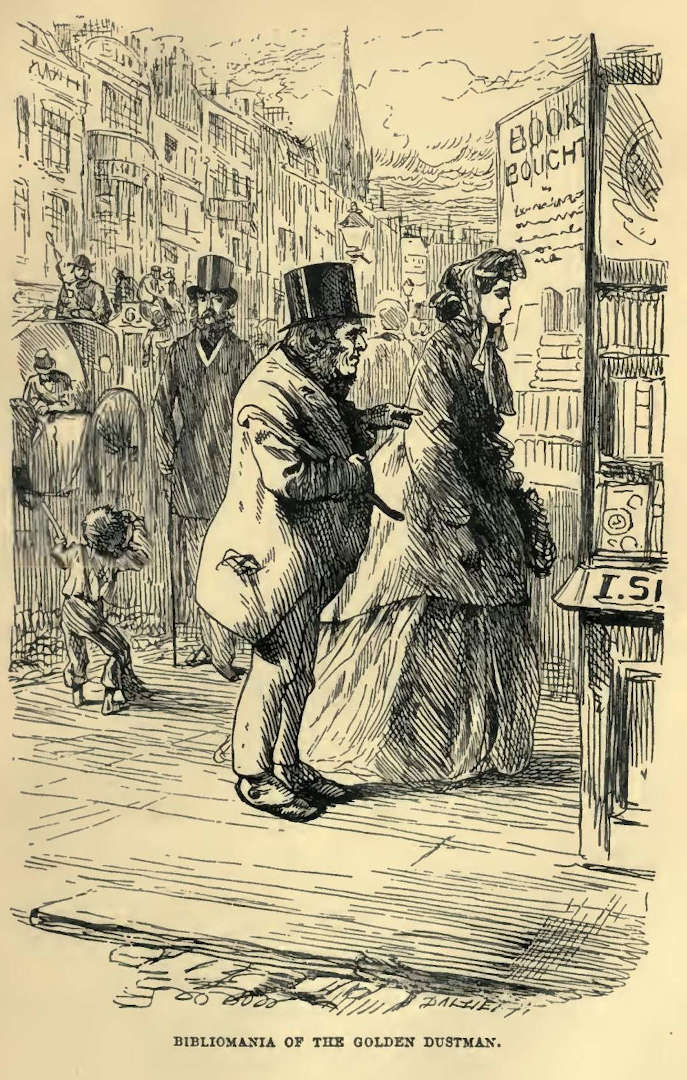
\includegraphics[scale=2.3]{03-05-01}

Chapter 3

THE GOLDEN DUSTMAN SINKS AGAIN


The evening of that day being one of the reading evenings at the Bower,
Mr Boffin kissed Mrs Boffin after a five o’clock dinner, and trotted
out, nursing his big stick in both arms, so that, as of old, it seemed
to be whispering in his ear. He carried so very attentive an expression
on his countenance that it appeared as if the confidential discourse of
the big stick required to be followed closely. Mr Boffin’s face was like
the face of a thoughtful listener to an intricate communication, and, in
trotting along, he occasionally glanced at that companion with the look
of a man who was interposing the remark: ‘You don’t mean it!’

Mr Boffin and his stick went on alone together, until they arrived at
certain cross-ways where they would be likely to fall in with any one
coming, at about the same time, from Clerkenwell to the Bower. Here they
stopped, and Mr Boffin consulted his watch.

‘It wants five minutes, good, to Venus’s appointment,’ said he. ‘I’m
rather early.’

But Venus was a punctual man, and, even as Mr Boffin replaced his watch
in its pocket, was to be descried coming towards him. He quickened his
pace on seeing Mr Boffin already at the place of meeting, and was soon
at his side.

‘Thank’ee, Venus,’ said Mr Boffin. ‘Thank’ee, thank’ee, thank’ee!’

It would not have been very evident why he thanked the anatomist, but
for his furnishing the explanation in what he went on to say.

‘All right, Venus, all right. Now, that you’ve been to see me, and have
consented to keep up the appearance before Wegg of remaining in it for a
time, I have got a sort of a backer. All right, Venus. Thank’ee, Venus.
Thank’ee, thank’ee, thank’ee!’

Mr Venus shook the proffered hand with a modest air, and they pursued
the direction of the Bower.

‘Do you think Wegg is likely to drop down upon me to-night, Venus?’
inquired Mr Boffin, wistfully, as they went along.

‘I think he is, sir.’

‘Have you any particular reason for thinking so, Venus?’

‘Well, sir,’ returned that personage, ‘the fact is, he has given me
another look-in, to make sure of what he calls our stock-in-trade being
correct, and he has mentioned his intention that he was not to be put
off beginning with you the very next time you should come. And this,’
hinted Mr Venus, delicately, ‘being the very next time, you know, sir--’

--‘Why, therefore you suppose he’ll turn to at the grindstone, eh,
Wegg?’ said Mr Boffin.

‘Just so, sir.’

Mr Boffin took his nose in his hand, as if it were already excoriated,
and the sparks were beginning to fly out of that feature. ‘He’s a
terrible fellow, Venus; he’s an awful fellow. I don’t know how ever I
shall go through with it. You must stand by me, Venus like a good man
and true. You’ll do all you can to stand by me, Venus; won’t you?’

Mr Venus replied with the assurance that he would; and Mr Boffin,
looking anxious and dispirited, pursued the way in silence until they
rang at the Bower gate. The stumping approach of Wegg was soon heard
behind it, and as it turned upon its hinges he became visible with his
hand on the lock.

‘Mr Boffin, sir?’ he remarked. ‘You’re quite a stranger!’

‘Yes. I’ve been otherwise occupied, Wegg.’

‘Have you indeed, sir?’ returned the literary gentleman, with a
threatening sneer. ‘Hah! I’ve been looking for you, sir, rather what I
may call specially.’

‘You don’t say so, Wegg?’

‘Yes, I do say so, sir. And if you hadn’t come round to me tonight, dash
my wig if I wouldn’t have come round to you tomorrow. Now! I tell you!’

‘Nothing wrong, I hope, Wegg?’

‘Oh no, Mr Boffin,’ was the ironical answer. ‘Nothing wrong! What should
be wrong in Boffinses Bower! Step in, sir.’

     ‘“If you’ll come to the Bower I’ve shaded for you,
     Your bed shan’t be roses all spangled with doo:
     Will you, will you, will you, will you, come to the Bower?
     Oh, won’t you, won’t you, won’t you, won’t you, come to the
          Bower?”’

An unholy glare of contradiction and offence shone in the eyes of Mr
Wegg, as he turned the key on his patron, after ushering him into the
yard with this vocal quotation. Mr Boffin’s air was crestfallen and
submissive. Whispered Wegg to Venus, as they crossed the yard behind
him: ‘Look at the worm and minion; he’s down in the mouth already.’
Whispered Venus to Wegg: ‘That’s because I’ve told him. I’ve prepared
the way for you.’

Mr Boffin, entering the usual chamber, laid his stick upon the settle
usually reserved for him, thrust his hands into his pockets, and,
with his shoulders raised and his hat drooping back upon them, looking
disconsolately at Wegg. ‘My friend and partner, Mr Venus, gives me to
understand,’ remarked that man of might, addressing him, ‘that you are
aware of our power over you. Now, when you have took your hat off, we’ll
go into that pint.’

Mr Boffin shook it off with one shake, so that it dropped on the floor
behind him, and remained in his former attitude with his former rueful
look upon him.

‘First of all, I’m a-going to call you Boffin, for short,’ said Wegg.
‘If you don’t like it, it’s open to you to lump it.’

‘I don’t mind it, Wegg,’ Mr Boffin replied.

‘That’s lucky for you, Boffin. Now, do you want to be read to?’

‘I don’t particularly care about it to-night, Wegg.’

‘Because if you did want to,’ pursued Mr Wegg, the brilliancy of whose
point was dimmed by his having been unexpectedly answered: ‘you wouldn’t
be. I’ve been your slave long enough. I’m not to be trampled under-foot
by a dustman any more. With the single exception of the salary, I
renounce the whole and total sitiwation.’

‘Since you say it is to be so, Wegg,’ returned Mr Boffin, with folded
hands, ‘I suppose it must be.’

‘I suppose it must be,’ Wegg retorted. ‘Next (to clear the ground before
coming to business), you’ve placed in this yard a skulking, a sneaking,
and a sniffing, menial.’

‘He hadn’t a cold in his head when I sent him here,’ said Mr Boffin.

‘Boffin!’ retorted Wegg, ‘I warn you not to attempt a joke with me!’

Here Mr Venus interposed, and remarked that he conceived Mr Boffin to
have taken the description literally; the rather, forasmuch as he, Mr
Venus, had himself supposed the menial to have contracted an affliction
or a habit of the nose, involving a serious drawback on the pleasures of
social intercourse, until he had discovered that Mr Wegg’s description
of him was to be accepted as merely figurative.

‘Anyhow, and every how,’ said Wegg, ‘he has been planted here, and he
is here. Now, I won’t have him here. So I call upon Boffin, before I say
another word, to fetch him in and send him packing to the right-about.’

The unsuspecting Sloppy was at that moment airing his many buttons
within view of the window. Mr Boffin, after a short interval of
impassive discomfiture, opened the window and beckoned him to come in.

‘I call upon Boffin,’ said Wegg, with one arm a-kimbo and his head on
one side, like a bullying counsel pausing for an answer from a witness,
‘to inform that menial that I am Master here!’

In humble obedience, when the button-gleaming Sloppy entered Mr Boffin
said to him: ‘Sloppy, my fine fellow, Mr Wegg is Master here. He doesn’t
want you, and you are to go from here.’

‘For good!’ Mr Wegg severely stipulated.

‘For good,’ said Mr Boffin.

Sloppy stared, with both his eyes and all his buttons, and his mouth
wide open; but was without loss of time escorted forth by Silas Wegg,
pushed out at the yard gate by the shoulders, and locked out.

‘The atomspear,’ said Wegg, stumping back into the room again, a
little reddened by his late exertion, ‘is now freer for the purposes of
respiration. Mr Venus, sir, take a chair. Boffin, you may sit down.’

Mr Boffin, still with his hands ruefully stuck in his pockets, sat on
the edge of the settle, shrunk into a small compass, and eyed the potent
Silas with conciliatory looks.

‘This gentleman,’ said Silas Wegg, pointing out Venus, ‘this gentleman,
Boffin, is more milk and watery with you than I’ll be. But he hasn’t
borne the Roman yoke as I have, nor yet he hasn’t been required to
pander to your depraved appetite for miserly characters.’

‘I never meant, my dear Wegg--’ Mr Boffin was beginning, when Silas
stopped him.

‘Hold your tongue, Boffin! Answer when you’re called upon to answer.
You’ll find you’ve got quite enough to do. Now, you’re aware--are
you--that you’re in possession of property to which you’ve no right at
all? Are you aware of that?’

‘Venus tells me so,’ said Mr Boffin, glancing towards him for any
support he could give.

‘I tell you so,’ returned Silas. ‘Now, here’s my hat, Boffin, and here’s
my walking-stick. Trifle with me, and instead of making a bargain with
you, I’ll put on my hat and take up my walking-stick, and go out, and
make a bargain with the rightful owner. Now, what do you say?’

‘I say,’ returned Mr Boffin, leaning forward in alarmed appeal, with his
hands on his knees, ‘that I am sure I don’t want to trifle. Wegg. I have
said so to Venus.’

‘You certainly have, sir,’ said Venus.

‘You’re too milk and watery with our friend, you are indeed,’
remonstrated Silas, with a disapproving shake of his wooden head. ‘Then
at once you confess yourself desirous to come to terms, do you Boffin?
Before you answer, keep this hat well in your mind and also this
walking-stick.’

‘I am willing, Wegg, to come to terms.’

‘Willing won’t do, Boffin. I won’t take willing. Are you desirous to
come to terms? Do you ask to be allowed as a favour to come to terms?’
Mr Wegg again planted his arm, and put his head on one side.

‘Yes.’

‘Yes what?’ said the inexorable Wegg: ‘I won’t take yes. I’ll have it
out of you in full, Boffin.’

‘Dear me!’ cried that unfortunate gentleman. ‘I am so worrited! I ask to
be allowed to come to terms, supposing your document is all correct.’

‘Don’t you be afraid of that,’ said Silas, poking his head at him. ‘You
shall be satisfied by seeing it. Mr Venus will show it you, and I’ll
hold you the while. Then you want to know what the terms are. Is
that about the sum and substance of it? Will you or won’t you answer,
Boffin?’ For he had paused a moment.

‘Dear me!’ cried that unfortunate gentleman again, ‘I am worrited to
that degree that I’m almost off my head. You hurry me so. Be so good as
name the terms, Wegg.’

‘Now, mark, Boffin,’ returned Silas: ‘Mark ‘em well, because they’re
the lowest terms and the only terms. You’ll throw your Mound (the little
Mound as comes to you any way) into the general estate, and then you’ll
divide the whole property into three parts, and you’ll keep one and hand
over the others.’

Mr Venus’s mouth screwed itself up, as Mr Boffin’s face lengthened
itself, Mr Venus not having been prepared for such a rapacious demand.

‘Now, wait a bit, Boffin,’ Wegg proceeded, ‘there’s something more.
You’ve been a squandering this property--laying some of it out on
yourself. THAT won’t do. You’ve bought a house. You’ll be charged for
it.’

‘I shall be ruined, Wegg!’ Mr Boffin faintly protested.

‘Now, wait a bit, Boffin; there’s something more. You’ll leave me in
sole custody of these Mounds till they’re all laid low. If any waluables
should be found in ‘em, I’ll take care of such waluables. You’ll produce
your contract for the sale of the Mounds, that we may know to a penny
what they’re worth, and you’ll make out likewise an exact list of
all the other property. When the Mounds is cleared away to the last
shovel-full, the final diwision will come off.’

‘Dreadful, dreadful, dreadful! I shall die in a workhouse!’ cried the
Golden Dustman, with his hands to his head.

‘Now, wait a bit, Boffin; there’s something more. You’ve been unlawfully
ferreting about this yard. You’ve been seen in the act of ferreting
about this yard. Two pair of eyes at the present moment brought to bear
upon you, have seen you dig up a Dutch bottle.’

‘It was mine, Wegg,’ protested Mr Boffin. ‘I put it there myself.’

‘What was in it, Boffin?’ inquired Silas.

‘Not gold, not silver, not bank notes, not jewels, nothing that you
could turn into money, Wegg; upon my soul!’

‘Prepared, Mr Venus,’ said Wegg, turning to his partner with a knowing
and superior air, ‘for an ewasive answer on the part of our dusty friend
here, I have hit out a little idea which I think will meet your views.
We charge that bottle against our dusty friend at a thousand pound.’

Mr Boffin drew a deep groan.

‘Now, wait a bit, Boffin; there’s something more. In your employment
is an under-handed sneak, named Rokesmith. It won’t answer to have HIM
about, while this business of ours is about. He must be discharged.’

‘Rokesmith is already discharged,’ said Mr Boffin, speaking in a muffled
voice, with his hands before his face, as he rocked himself on the
settle.

‘Already discharged, is he?’ returned Wegg, surprised. ‘Oh! Then,
Boffin, I believe there’s nothing more at present.’

The unlucky gentleman continuing to rock himself to and fro, and to
utter an occasional moan, Mr Venus besought him to bear up against his
reverses, and to take time to accustom himself to the thought of his new
position. But, his taking time was exactly the thing of all others that
Silas Wegg could not be induced to hear of. ‘Yes or no, and no half
measures!’ was the motto which that obdurate person many times repeated;
shaking his fist at Mr Boffin, and pegging his motto into the floor with
his wooden leg, in a threatening and alarming manner.

At length, Mr Boffin entreated to be allowed a quarter of an hour’s
grace, and a cooling walk of that duration in the yard. With some
difficulty Mr Wegg granted this great favour, but only on condition
that he accompanied Mr Boffin in his walk, as not knowing what he might
fraudulently unearth if he were left to himself. A more absurd sight
than Mr Boffin in his mental irritation trotting very nimbly, and Mr
Wegg hopping after him with great exertion, eager to watch the slightest
turn of an eyelash, lest it should indicate a spot rich with some
secret, assuredly had never been seen in the shadow of the Mounds. Mr
Wegg was much distressed when the quarter of an hour expired, and came
hopping in, a very bad second.

‘I can’t help myself!’ cried Mr Boffin, flouncing on the settle in a
forlorn manner, with his hands deep in his pockets, as if his pockets
had sunk. ‘What’s the good of my pretending to stand out, when I can’t
help myself? I must give in to the terms. But I should like to see the
document.’

Wegg, who was all for clinching the nail he had so strongly driven home,
announced that Boffin should see it without an hour’s delay. Taking him
into custody for that purpose, or overshadowing him as if he really were
his Evil Genius in visible form, Mr Wegg clapped Mr Boffin’s hat
upon the back of his head, and walked him out by the arm, asserting a
proprietorship over his soul and body that was at once more grim and
more ridiculous than anything in Mr Venus’s rare collection. That
light-haired gentleman followed close upon their heels, at least backing
up Mr Boffin in a literal sense, if he had not had recent opportunities
of doing so spiritually; while Mr Boffin, trotting on as hard as he
could trot, involved Silas Wegg in frequent collisions with the public,
much as a pre-occupied blind man’s dog may be seen to involve his
master.

Thus they reached Mr Venus’s establishment, somewhat heated by the
nature of their progress thither. Mr Wegg, especially, was in a flaming
glow, and stood in the little shop, panting and mopping his head with
his pocket-handkerchief, speechless for several minutes.

Meanwhile, Mr Venus, who had left the duelling frogs to fight it out in
his absence by candlelight for the public delectation, put the shutters
up. When all was snug, and the shop-door fastened, he said to the
perspiring Silas: ‘I suppose, Mr Wegg, we may now produce the paper?’

‘Hold on a minute, sir,’ replied that discreet character; ‘hold on a
minute. Will you obligingly shove that box--which you mentioned on a
former occasion as containing miscellanies--towards me in the midst of
the shop here?’

Mr Venus did as he was asked.

‘Very good,’ said Silas, looking about: ‘ve--ry good. Will you hand me
that chair, sir, to put a-top of it?’

Venus handed him the chair.

‘Now, Boffin,’ said Wegg, ‘mount up here and take your seat, will you?’

Mr Boffin, as if he were about to have his portrait painted, or to be
electrified, or to be made a Freemason, or to be placed at any other
solitary disadvantage, ascended the rostrum prepared for him.

‘Now, Mr Venus,’ said Silas, taking off his coat, ‘when I catches our
friend here round the arms and body, and pins him tight to the back of
the chair, you may show him what he wants to see. If you’ll open it and
hold it well up in one hand, sir, and a candle in the other, he can read
it charming.’

Mr Boffin seemed rather inclined to object to these precautionary
arrangements, but, being immediately embraced by Wegg, resigned himself.
Venus then produced the document, and Mr Boffin slowly spelt it out
aloud: so very slowly, that Wegg, who was holding him in the chair
with the grip of a wrestler, became again exceedingly the worse for his
exertions. ‘Say when you’ve put it safe back, Mr Venus,’ he uttered with
difficulty, ‘for the strain of this is terrimenjious.’

At length the document was restored to its place; and Wegg, whose
uncomfortable attitude had been that of a very persevering man
unsuccessfully attempting to stand upon his head, took a seat to recover
himself. Mr Boffin, for his part, made no attempt to come down, but
remained aloft disconsolate.

‘Well, Boffin!’ said Wegg, as soon as he was in a condition to speak.
‘Now, you know.’

‘Yes, Wegg,’ said Mr Boffin, meekly. ‘Now, I know.’

‘You have no doubts about it, Boffin.’

‘No, Wegg. No, Wegg. None,’ was the slow and sad reply.

‘Then, take care, you,’ said Wegg, ‘that you stick to your conditions.
Mr Venus, if on this auspicious occasion, you should happen to have a
drop of anything not quite so mild as tea in the ‘ouse, I think I’d take
the friendly liberty of asking you for a specimen of it.’

Mr Venus, reminded of the duties of hospitality, produced some rum.
In answer to the inquiry, ‘Will you mix it, Mr Wegg?’ that gentleman
pleasantly rejoined, ‘I think not, sir. On so auspicious an occasion, I
prefer to take it in the form of a Gum-Tickler.’

Mr Boffin, declining rum, being still elevated on his pedestal, was in
a convenient position to be addressed. Wegg having eyed him with an
impudent air at leisure, addressed him, therefore, while refreshing
himself with his dram.

‘Bof--fin!’

‘Yes, Wegg,’ he answered, coming out of a fit of abstraction, with a
sigh.

‘I haven’t mentioned one thing, because it’s a detail that comes of
course. You must be followed up, you know. You must be kept under
inspection.’

‘I don’t quite understand,’ said Mr Boffin.

‘Don’t you?’ sneered Wegg. ‘Where’s your wits, Boffin? Till the Mounds
is down and this business completed, you’re accountable for all the
property, recollect. Consider yourself accountable to me. Mr Venus here
being too milk and watery with you, I am the boy for you.’

‘I’ve been a-thinking,’ said Mr Boffin, in a tone of despondency, ‘that
I must keep the knowledge from my old lady.’

‘The knowledge of the diwision, d’ye mean?’ inquired Wegg, helping
himself to a third Gum-Tickler--for he had already taken a second.

‘Yes. If she was to die first of us two she might then think all her
life, poor thing, that I had got the rest of the fortune still, and was
saving it.’

‘I suspect, Boffin,’ returned Wegg, shaking his head sagaciously, and
bestowing a wooden wink upon him, ‘that you’ve found out some account
of some old chap, supposed to be a Miser, who got himself the credit of
having much more money than he had. However, I don’t mind.’

‘Don’t you see, Wegg?’ Mr Boffin feelingly represented to him: ‘don’t
you see? My old lady has got so used to the property. It would be such a
hard surprise.’

‘I don’t see it at all,’ blustered Wegg. ‘You’ll have as much as I
shall. And who are you?’

‘But then, again,’ Mr Boffin gently represented; ‘my old lady has very
upright principles.’

‘Who’s your old lady,’ returned Wegg, ‘to set herself up for having
uprighter principles than mine?’

Mr Boffin seemed a little less patient at this point than at any other
of the negotiations. But he commanded himself, and said tamely enough:
‘I think it must be kept from my old lady, Wegg.’

‘Well,’ said Wegg, contemptuously, though, perhaps, perceiving some hint
of danger otherwise, ‘keep it from your old lady. I ain’t going to tell
her. I can have you under close inspection without that. I’m as good a
man as you, and better. Ask me to dinner. Give me the run of your ‘ouse.
I was good enough for you and your old lady once, when I helped you out
with your weal and hammers. Was there no Miss Elizabeth, Master George,
Aunt Jane, and Uncle Parker, before YOU two?’

‘Gently, Mr Wegg, gently,’ Venus urged.

‘Milk and water-erily you mean, sir,’ he returned, with some little
thickness of speech, in consequence of the Gum-Ticklers having tickled
it. ‘I’ve got him under inspection, and I’ll inspect him.

     “Along the line the signal ran
     England expects as this present man
     Will keep Boffin to his duty.”

--Boffin, I’ll see you home.’

Mr Boffin descended with an air of resignation, and gave himself up,
after taking friendly leave of Mr Venus. Once more, Inspector and
Inspected went through the streets together, and so arrived at Mr
Boffin’s door.

But even there, when Mr Boffin had given his keeper good-night, and had
let himself in with his key, and had softly closed the door, even there
and then, the all-powerful Silas must needs claim another assertion of
his newly-asserted power.

‘Bof--fin!’ he called through the keyhole.

‘Yes, Wegg,’ was the reply through the same channel.

‘Come out. Show yourself again. Let’s have another look at you!’
Mr Boffin--ah, how fallen from the high estate of his honest
simplicity!--opened the door and obeyed.

‘Go in. You may get to bed now,’ said Wegg, with a grin.

The door was hardly closed, when he again called through the keyhole:
‘Bof--fin!’

‘Yes, Wegg.’

This time Silas made no reply, but laboured with a will at turning an
imaginary grindstone outside the keyhole, while Mr Boffin stooped at it
within; he then laughed silently, and stumped home.



